\textbf{Solução:}
As árvores B+ e B* são extensões da árvore B. Ou seja, elas incorporam a maioria das características da árvore B, com exceção de:
\begin{itemize}
    \item \textbf{Árvore B+:} Os registros são armazenados apenas nas folhas, isto é, os nós internos (que não são folhas) guardam apenas algumas chaves. Além disso, as folhas são encadeadas para acesso sequencial. Veja, por exemplo, a \autoref{fig:b_plus_tree}. Nela, não estão representados os registros, claramente, mas, se estivessem, estariam apenas nas folhas. Porém, podemos ver que algumas chaves presentes nas folhas são repetidas nos nós internos; isso acontece com a primeira chave de cada nó folha. O que é interessante sobre essa árvore é que, dado que possuímos acesso ao nó que contém as chaves 25 e 28, por exemplo, é trivial avançar para o nó que contém as próximas chaves 30 e 35. Outras diferenças da árvore B+ com relação à árvore B são os algoritmos de busca, inserção e remoção, que são adaptados para lidar com essas novas características.
    \begin{figure}[H]
        \centering
        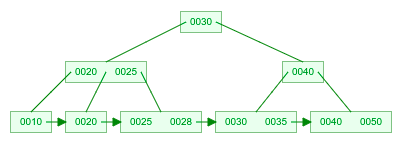
\includegraphics[width=0.5\linewidth]{b_plus_tree.png}
        \caption{Exemplo de árvore B+. Criado com a ferramenta B+ Tree Visualization\protect\footnotemark, da University of San Francisco.}
        \label{fig:b_plus_tree}
    \end{figure}
    \footnotetext{Disponível em \href{https://www.cs.usfca.edu/~galles/visualization/BPlusTree.html}{https://www.cs.usfca.edu/~galles/visualization/BPlusTree.html}.}
    \item \textbf{Árvore B*:} O objetivo dessa árvore é manter os nós internos os mais cheios possível. Isso é feito pedindo que os nós contenham no mínimo 2/3 da sua capacidade, ao invés de 1/2, como na árvore B. Além disso, os algoritmos de inserção e remoção são modificados. Por exemplo, ao invés de simplesmente dividir um nó quando ele está cheio, busca-se redistribuir as chaves com os irmãos, evitando o custo de divisão de nós.
\end{itemize}
